%% Creator: Inkscape inkscape 0.92.2, www.inkscape.org
%% PDF/EPS/PS + LaTeX output extension by Johan Engelen, 2010
%% Accompanies image file 'fle5.eps' (pdf, eps, ps)
%%
%% To include the image in your LaTeX document, write
%%   \input{<filename>.pdf_tex}
%%  instead of
%%   \includegraphics{<filename>.pdf}
%% To scale the image, write
%%   \def\svgwidth{<desired width>}
%%   \input{<filename>.pdf_tex}
%%  instead of
%%   \includegraphics[width=<desired width>]{<filename>.pdf}
%%
%% Images with a different path to the parent latex file can
%% be accessed with the `import' package (which may need to be
%% installed) using
%%   \usepackage{import}
%% in the preamble, and then including the image with
%%   \import{<path to file>}{<filename>.pdf_tex}
%% Alternatively, one can specify
%%   \graphicspath{{<path to file>/}}
%% 
%% For more information, please see info/svg-inkscape on CTAN:
%%   http://tug.ctan.org/tex-archive/info/svg-inkscape
%%
\begingroup%
  \makeatletter%
  \providecommand\color[2][]{%
    \errmessage{(Inkscape) Color is used for the text in Inkscape, but the package 'color.sty' is not loaded}%
    \renewcommand\color[2][]{}%
  }%
  \providecommand\transparent[1]{%
    \errmessage{(Inkscape) Transparency is used (non-zero) for the text in Inkscape, but the package 'transparent.sty' is not loaded}%
    \renewcommand\transparent[1]{}%
  }%
  \providecommand\rotatebox[2]{#2}%
  \ifx\svgwidth\undefined%
    \setlength{\unitlength}{344.79999138bp}%
    \ifx\svgscale\undefined%
      \relax%
    \else%
      \setlength{\unitlength}{\unitlength * \real{\svgscale}}%
    \fi%
  \else%
    \setlength{\unitlength}{\svgwidth}%
  \fi%
  \global\let\svgwidth\undefined%
  \global\let\svgscale\undefined%
  \makeatother%
  \begin{picture}(1,0.83526682)%
    \put(0,0){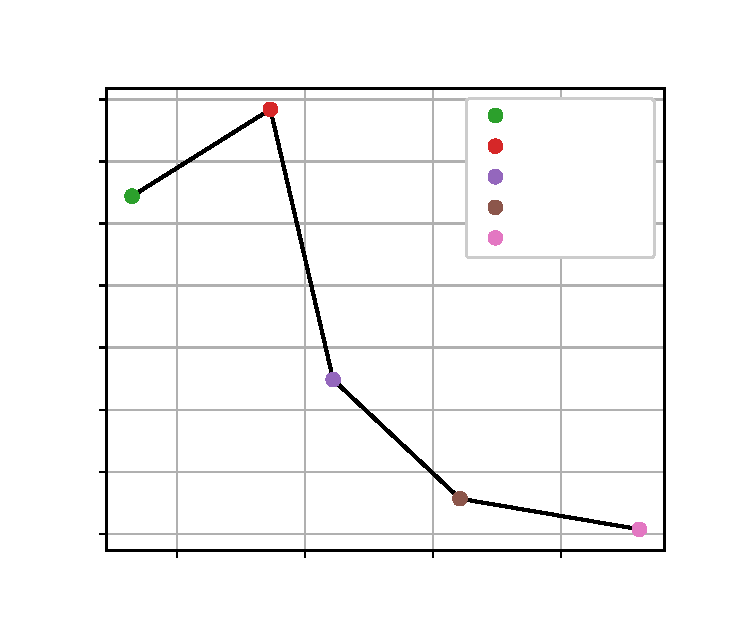
\includegraphics[width=\unitlength]{images_2ddl/fle5.eps}}%
    \put(0.20458643,0.04955423){\color[rgb]{0,0,0}\makebox(0,0)[lb]{\smash{10}}}%
    \put(0.38291183,0.04955423){\color[rgb]{0,0,0}\makebox(0,0)[lb]{\smash{20}}}%
    \put(0.5612355,0.04955423){\color[rgb]{0,0,0}\makebox(0,0)[lb]{\smash{30}}}%
    \put(0.73955916,0.04955423){\color[rgb]{0,0,0}\makebox(0,0)[lb]{\smash{40\\ r_1 (mm)}}}%
    \put(0.05885673,0.10360499){\color[rgb]{0,0,0}\makebox(0,0)[lb]{\smash{0.0}}}%
    \put(0.05885673,0.19000493){\color[rgb]{0,0,0}\makebox(0,0)[lb]{\smash{0.1}}}%
    \put(0.05885673,0.27640574){\color[rgb]{0,0,0}\makebox(0,0)[lb]{\smash{0.2}}}%
    \put(0.05885673,0.36280742){\color[rgb]{0,0,0}\makebox(0,0)[lb]{\smash{0.3}}}%
    \put(0.05885673,0.44920534){\color[rgb]{0,0,0}\makebox(0,0)[lb]{\smash{0.4}}}%
    \put(0.05885673,0.53560615){\color[rgb]{0,0,0}\makebox(0,0)[lb]{\smash{0.5}}}%
    \put(0.05885673,0.62200696){\color[rgb]{0,0,0}\makebox(0,0)[lb]{\smash{0.6}}}%
    \put(0.05885673,0.70840777){\color[rgb]{0,0,0}\makebox(0,0)[lb]{\smash{0.7}}}%
    \put(0.04041299,0.33361079){\color[rgb]{0,0,0}\rotatebox{90}{\makebox(0,0)[lb]{\smash{H_max (m)}}}}%
    \put(0.16366705,0.75243619){\color[rgb]{0,0,0}\makebox(0,0)[lb]{\smash{écoulement saut pieds joints: F=4500N }}}%
    \put(0.71864849,0.68690835){\color[rgb]{0,0,0}\makebox(0,0)[lb]{\smash{r2=15 mm}}}%
    \put(0.71864849,0.64435615){\color[rgb]{0,0,0}\makebox(0,0)[lb]{\smash{r2=20 mm}}}%
    \put(0.71864849,0.60180394){\color[rgb]{0,0,0}\makebox(0,0)[lb]{\smash{r2=25 mm}}}%
    \put(0.71864849,0.55925174){\color[rgb]{0,0,0}\makebox(0,0)[lb]{\smash{r2=35 mm}}}%
    \put(0.71864849,0.51670244){\color[rgb]{0,0,0}\makebox(0,0)[lb]{\smash{r2=50 mm}}}%
  \end{picture}%
\endgroup%
